\documentclass[]{nsm-thesis}
% options:
% [germanthesis] - Thesis is written in German
% [plainunnumbered] - Don't print numbers on plain pages
% [earlydraft] - Settings for quick draft printouts
% [watermark] - Print current time/date at bottom of each page
% [phdthesis] - switch to PhD thesis style
% [twoside] - double sided
% [cutmargins] - text body fills complete page

% Author name. Separate multiple authors with commas.
\author{Dmitriy Monakhov}
\birthday{28. April 1999}
\birthplace{Moscow}

% Title of your thesis.
\title{Improving Urban Traffic Flow with Drone Supported Vehicular Networks}

\thesistype{Master's Thesis in Distributed Systems Engineering}\thesiscite{Master's Thesis~(Masterarbeit)}

\advisors{Mario Franke}
% List of advisors (without academic titles), separated by commas.

% List of referees (without academic titles), separated by commas.
\referees{Christoph Sommer, Burkhard Hensel}


% Define abbreviations used in the thesis here.
%\acrodef{WSN}{Wireless Sensor Network}
\acrodef{MANET}{Mobile Ad Hoc Network}
\acrodef{VANET}{Vehicular Ad Hoc Network}
\acrodef{OSG}{OpenSceneGraph}
\acrodef{MAC}{Medium access control}
%\acrodef{ROI}{Region of Interest}{short-indefinite={an}, long-plural-form={Regions of Interest}}
%\acrodef{ADAC}{German Automobile Association}{foreign={Allgemeiner Deutscher Automobilclub}}
%\acrodef{CANhashing}[CAN]{Content Addressable Network}{extra={when referring to the distributed hash table}}
%\acrodef{CANproto}[CAN]{Controller Area Network}{extra={when referring to the bus protocol}}

\begin{document}

\pagenumbering{roman}

\maketitle

\cleardoublepage


\chapter*{Abstract}
\addcontentsline{toc}{chapter}{Abstract}
\begin{otherlanguage*}{american}

\TODO{Write abstract}

about 1/2 page:
\begin{enumerate}
    \item Motivation (Why do we care?)
    \item Problem statement (What problem are we trying to solve?)
    \item Approach (How did we go about it)
    \item Results (What's the answer?)
    \item Conclusion (What are the implications of the answer?)
\end{enumerate}

The abstract is a miniature version of the thesis.
It should be treated as an entirely separate document.
Do not assume that a reader who has access to an abstract will also have access to the thesis.
Do not assume that a reader who reads the thesis has read the abstract.

\end{otherlanguage*}


\chapter*{Kurzfassung}
\addcontentsline{toc}{chapter}{Kurzfassung}
\begin{otherlanguage*}{ngerman}

\TODO{Write short version of the Abstract in German?}
Gleicher Text (sinngemäß, nicht wörtlich) in Deutsch

\end{otherlanguage*}
\acresetall

\cleardoublepage
\tableofcontents
\TODO{The table of contents should fit on one page. When in doubt, adjust the \texttt{tocdepth} counter.}

\cleardoublepage
\pagenumbering{arabic}



\chapter{Introduction}
%\chapter{Einleitung}
\label{sec:introduction}

Current technology already enables us to create semi-autonomous vehicles. For now fully-autonomous vehicles are rarely allowed to 
populate the roads, in future it will probably be possible. One perspective option for autonomous driving are cooperative autonomous vehicles: such machines
that can drive on their own and maintain situation-awareness via communicating with other vehicles on the roads.

Since our world is rapidly urbanizing, it will be desirable to enable autonomous vehicles to drive in large cities. And there is a problem here: communication between cars will be difficult in urban areas. In cities, buildings stand close to each other. Buildings are usually built of radio-transparent materials. At the same time, the buildings are quite massive. Thus, it turns out that the propagation of radio signals between low-power car transmitters becomes very difficult if the cars are not on the same street. This leads to communication outages in vehicle-to-vehicles networks operating inside urban areas.

One possible solution to this problem could be drones. Cities of the future will probably be populated by autonomous drones flying in the air above the roofs of buildings. This gives drones the advantage of making it much easier for them to maintain a line of sight between each other and with vehicles on the ground. Consequently, their radio transmissions are less likely to be blocked by buildings. In this way, drones can help vehicles spread signals bypassing buildings standing between the vehicles.

In this paper, I explore whether there is an advantage in connecting a network of drones to a network of cars in terms of assisting with urban vehicular traffic.
Since a real-life experiment will be too expensive and difficult to conduct, I will use software simulation.

\chapter{Fundamentals}
\label{sec:fundamentals}

Before the beginning of the work, I will explain the basic terms, technologies and methods that will be used later. I see the Ad-hoc networks as a good starting point.

\section{Ad hoc networks}

A good definition of ad hoc networks was given by Ram Ramanathan and Jason Redi in IEEE communications Magazine \cite{ramanathan2002brief}: An ad hoc network is a (possibly mobile) collection of communications devices (nodes) that wish to communicate, but have no fixed infrastructure available, and have no pre-determined organization of available links. The authors further make a good point, stating that individual nodes are responsible for dynamically discovering which other nodes they can directly communicate with and the nodes are required to relay packets on behalf of other nodes in order to deliver data across the network.

According to Toor et al \cite{toor2008}, Vehicular ad hoc network (\ac{VANET}) is a special case of a mobile ad hoc network, where communication links are formed between the vehicles.

\section{Broadcast Storm}

A common challenge in implementing mobile ad hoc networks (including \acp{VANET}), according to \textcite{wisitrophan2007} is the broadcast storm. Authors define the broadcast storm as a frequent contention and collisions in transmission among neighboring nodes, when the nodes unconditionally broadcast packets. Authors further argue, that multiple solutions exist to alleviate this problem in usual \ac{MANET} environment, but only few are suitable to resolve the broadcast storm issue in \ac{VANET} context.

In my work the broadcast storm is also an issue that needs to be addressed. In my scenario the broadcast storm would be observed between vehicles and between drones if no suppression technique is present. At first, I will list some of the techniques, explored by \textcite{wisitrophan2007} for vehicular ad hoc networks and choose the one that is suitable for my scenario.

\begin{itemize}

\item \textbf{Weighted p-Persistence Broadcasting} - upon receiving a packet from node \emph{i}, node \emph{j} checks the packet ID and rebroadcasts with probability $\rho_{ij}$ if it receives the packet for the first time; otherwise, it discards the packet. \cite[Page~88]{wisitrophan2007}.

\item \textbf{Slotted 1-Persistence Broadcasting} - upon receiving a packet, a node checks the packet ID and rebroadcasts with probability 1 at the assigned time slot, if it receives the packet for the first time and has not received any duplicates before the assigned time slot; otherwise, it discards the packet \cite[Page~88]{wisitrophan2007}.

\item \textbf{Slotted p-Persistence Broadcasting} - Upon receiving a packet, a node checks the packet ID and rebroadcasts with the pre-determined probability $\rho$ at the assigned time slot, if it receives the packet for the first time and has not received any duplicates before its assigned time slot; otherwise, it discards the packet \cite[Page~89]{wisitrophan2007}.

\end{itemize}

\textcite{wisitrophan2007} also discuss Received-Signal-Strength-Based broadcast suppression schemes, but since in my work it is assumed that the vehicles always know their exact location, these techniques are not relevant.

In my work I will use the Slotted 1-Persistence Broadcasting for both vehicles and drones, because it is the simplest to implement and it shows sufficient performance in my scenario. In fact, since my scenario consists of high-density urban grid of roads, the communication between vehicles is highly obstructed, hence the collisions and contention in vehicle-to-vehicle is minimal.

\section {Related Work}
\TODO{Related Work: merging \acp{VANET} and DroneNETs}

\section {Simulation Software}

As is was mentioned earlier, conducting a full-scale real-life experiment will be very expensive. Therefore a good idea is to use software to simulate the scenario and evaluate the results. 

There are multiple network simulators available on the market. A survey, conducted by \textcite{pan2008survey} contains a list of most popular tools:
\begin{itemize}
\item OPNET \cite[Page~5]{pan2008survey}
\item Network Simulator 2 \cite[Page~7]{pan2008survey}
\item Network Simulator 3 \cite[Page~8]{pan2008survey}
\item OMNeT++ \cite[Page~10]{pan2008survey}
\end{itemize}

The one most suitable for my purposes is the OMNeT++. It is free for academical usage, but the main reason why I chose it is the fact that Veins \cite{Sommer2019} is based on OMNeT++. Veins will be discussed in the next section.

According to \textcite[Page~2]{Varga2010}, OMNeT++ is a discrete-event simulator. According to the author, discrete-event simulator simulates a system whose state, defined by the state of all entities of the system, changes only at discrete points in time and the change of state is triggers by the occurrence of an event.

\section {Veins}

In order to simulate a hybrid network of drones and vehicles a network simulator is not enough. A combined solution is needed to create a realistic scenario consisting of vehicles, buildings and drones. The software must implement a combination of a network simulator and a traffic simulator. My solution is based on Veins by \textcite{Sommer2019}.

\begin{figure}
  	\caption{High-level architecture of Veins. Veins bridges OMNeT++ with SUMO traffic simulator to enable simulation of \acp{VANET} \cite{Sommer2019}}
	\centering
	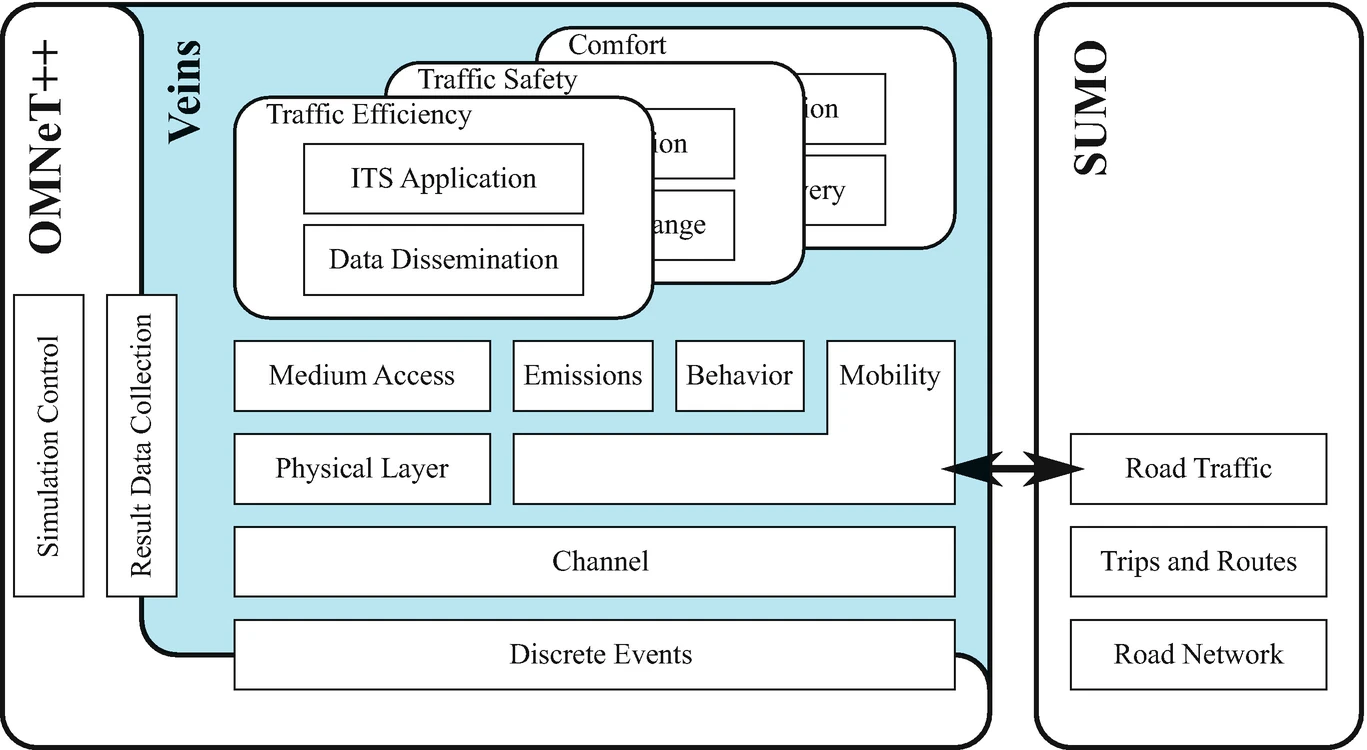
\includegraphics[width=1\textwidth]{figures/High-level Veins.png}
	\label{fig:veinshighlevel}
\end{figure}

\section{SUMO}
As shown on \ref{fig:veinshighlevel}, Veins uses SUMO by \textcite{sumo2018} as a traffic simulator. According to the SUMO developers, SUMO is a microscopic traffic simulator, which means that each vehicle and its dynamics are modeled individually.
This a suitable solution for my scenario, because I indeed need each vehicle to be an independent object with its own known position.

\section{Other software}

In addition to the Veins and SUMO I would like to emphasize the usage of OpenSceneGraph \cite{osg} as a 3D-rendering tool.  OMNeT++ natively supports OpenSceneGraph \cite{omnetpposg}, therefore \ac{OSG} is the most convenient and easy way to implement a 3D scene in OMNeT++. In this work, I will use 3D visualization for debugging purposes.

Veins provides a C++ class for \ac{OSG}-based road visualization. I will utilize this class along with my own vehicle-, drone- and building- visualizers.

\section{Simulated Hardware}

For my scenario the exact implementation of physical layer and \ac{MAC}-layer is not important. Therefore I am relying on networking, already implemented in Veins and OMNeT++. The physical layer is implemented by Veins and simulates Wi-Fi transmitter, mounted on the vehicle's roof (1.895 meters above the road). In my scenario, I use a monopole antenna, also already implemented by Veins. Since the transport-layer protocol is also not important, I am using Wave Short Message protocol, implemented in Veins. For the drones I use the same networking layers as for the vehicles.

\section {Scenario and Car}
\label{sec:scenarioned}

To further understand my implementation of drones in Veins, it is necessary to consider two files included in Veins: the file Scenario.ned \cite{scenarioned} and the file Car.ned \cite{carned}. Scenario.ned defines the overall structure of the network, contains an array of all nodes and a list of auxiliary modules that control the vehicles or participate in the visualization when working with the GUI. The Car.ned file defines the structure of one of the most important modules - Car module, which is the internal representation of a vehicle. It contains, in particular, information about the network controller simulator and information about the user code of the application. Also, the Car module has a sub-module, which is responsible for synchronizing the movement with SUMO. Based on these two files in the future I will implement my version of the scenario, which will include drones in addition to vehicles, as well as support three-dimensional visualization of the scene. 

\begin{figure}
  	\caption{Simplified diagram of Scenario \cite{scenarioned} network. Not all modules, parameters and connections are shown.}
	\centering
	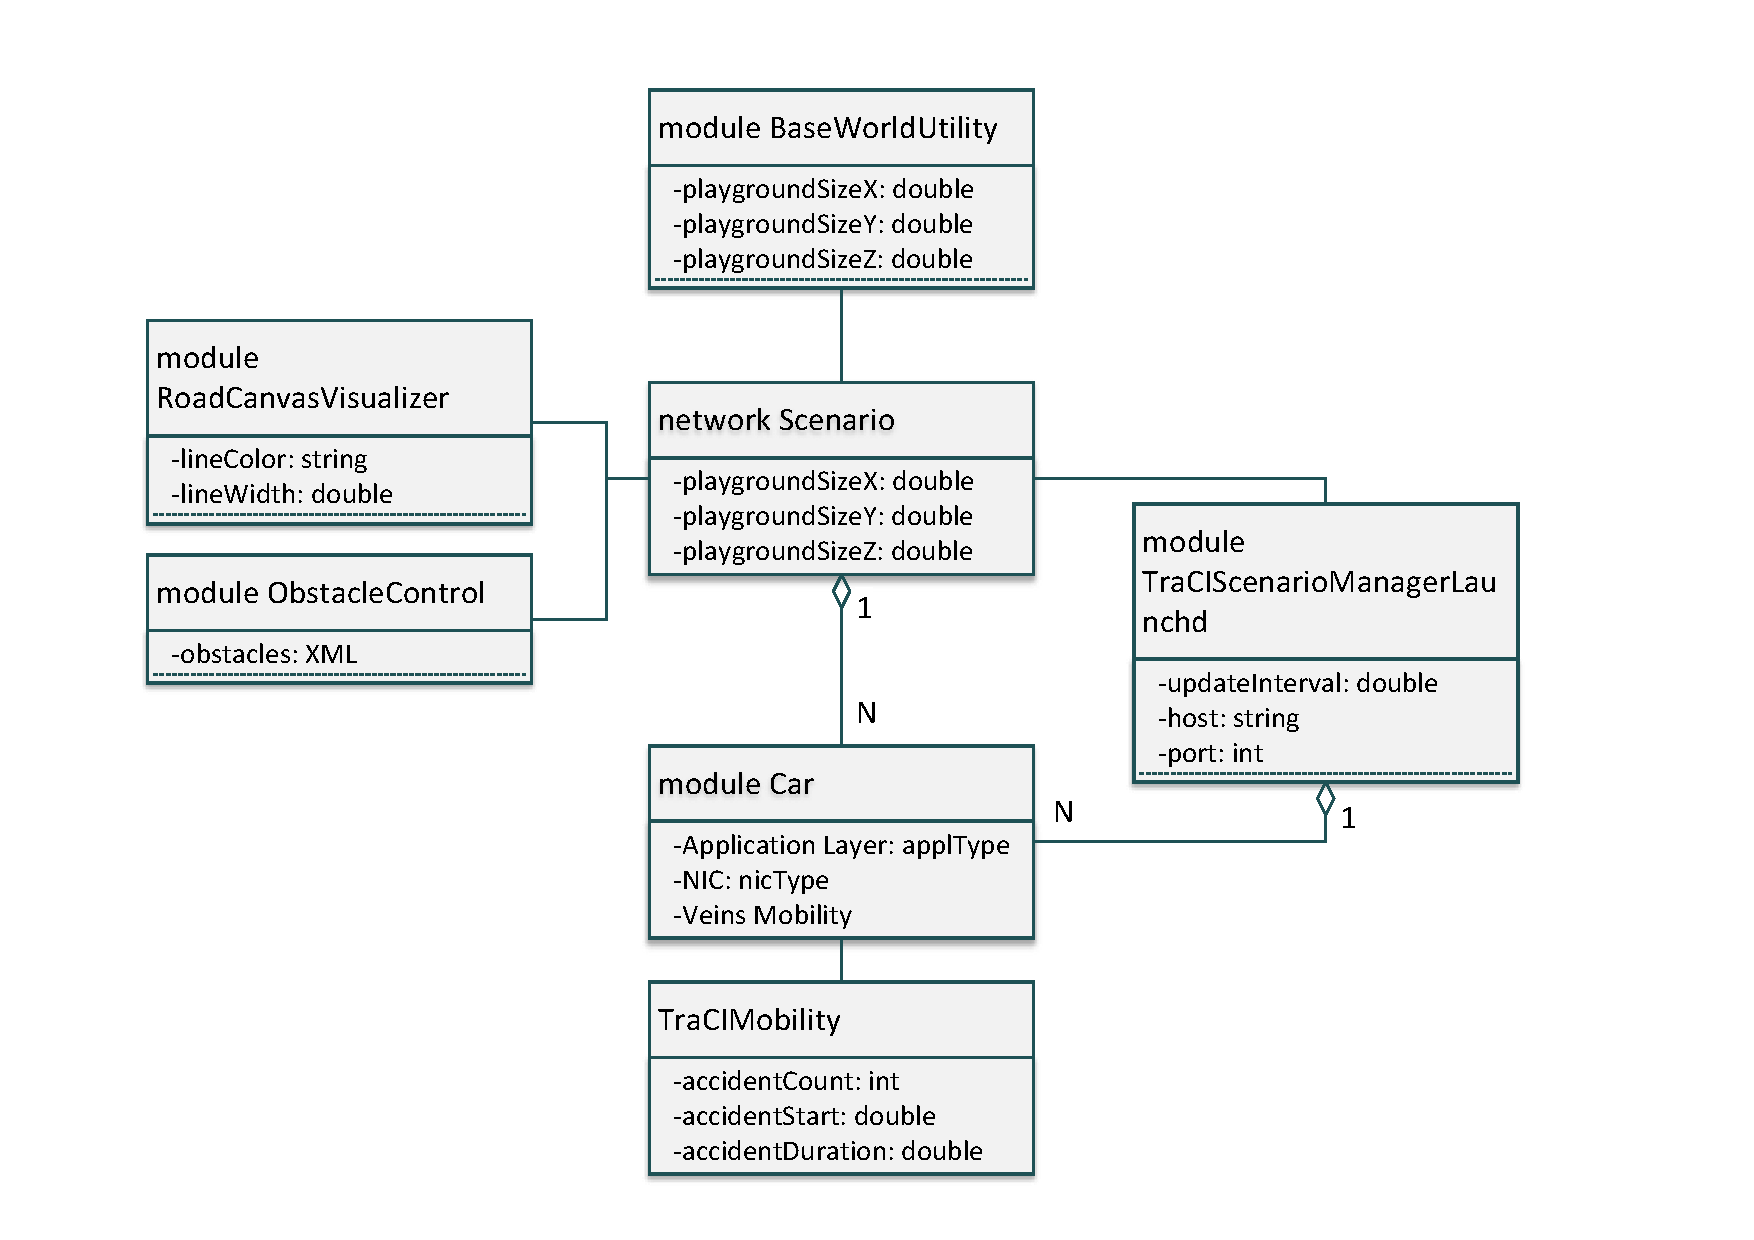
\includegraphics[width=1\textwidth]{figures/Scenario.pdf}
	\label{fig:scenarioned}
\end{figure}

\cref{fig:scenarioned} shows a simplified diagram of the network in Veins. It is not a diagram of classes in the usual sense, it shows the relationship of OMNeT++-modules and OMNeT++-networks , as well as some parameters that will be of interest in the rest of the work. 

\chapter{Implementation}

Now it is time to develop a network model for a scenario in which vehicles and drones will interact within the same virtual space. My implementation is largely based on the model used in Veins, which was discussed in \cref{sec:scenarioned}. My model basically repeats the structure of the model from Veins, as the basic modules remain the same. However, I have integrated into my model drones, support for the third dimension when calculating sight lines, and special modules for using OSG to render a three-dimensional scene.

\begin{figure}
  	\caption{Simplified diagram of DroneScenario network. Not all modules, parameters and connections are shown.}
	\centering
	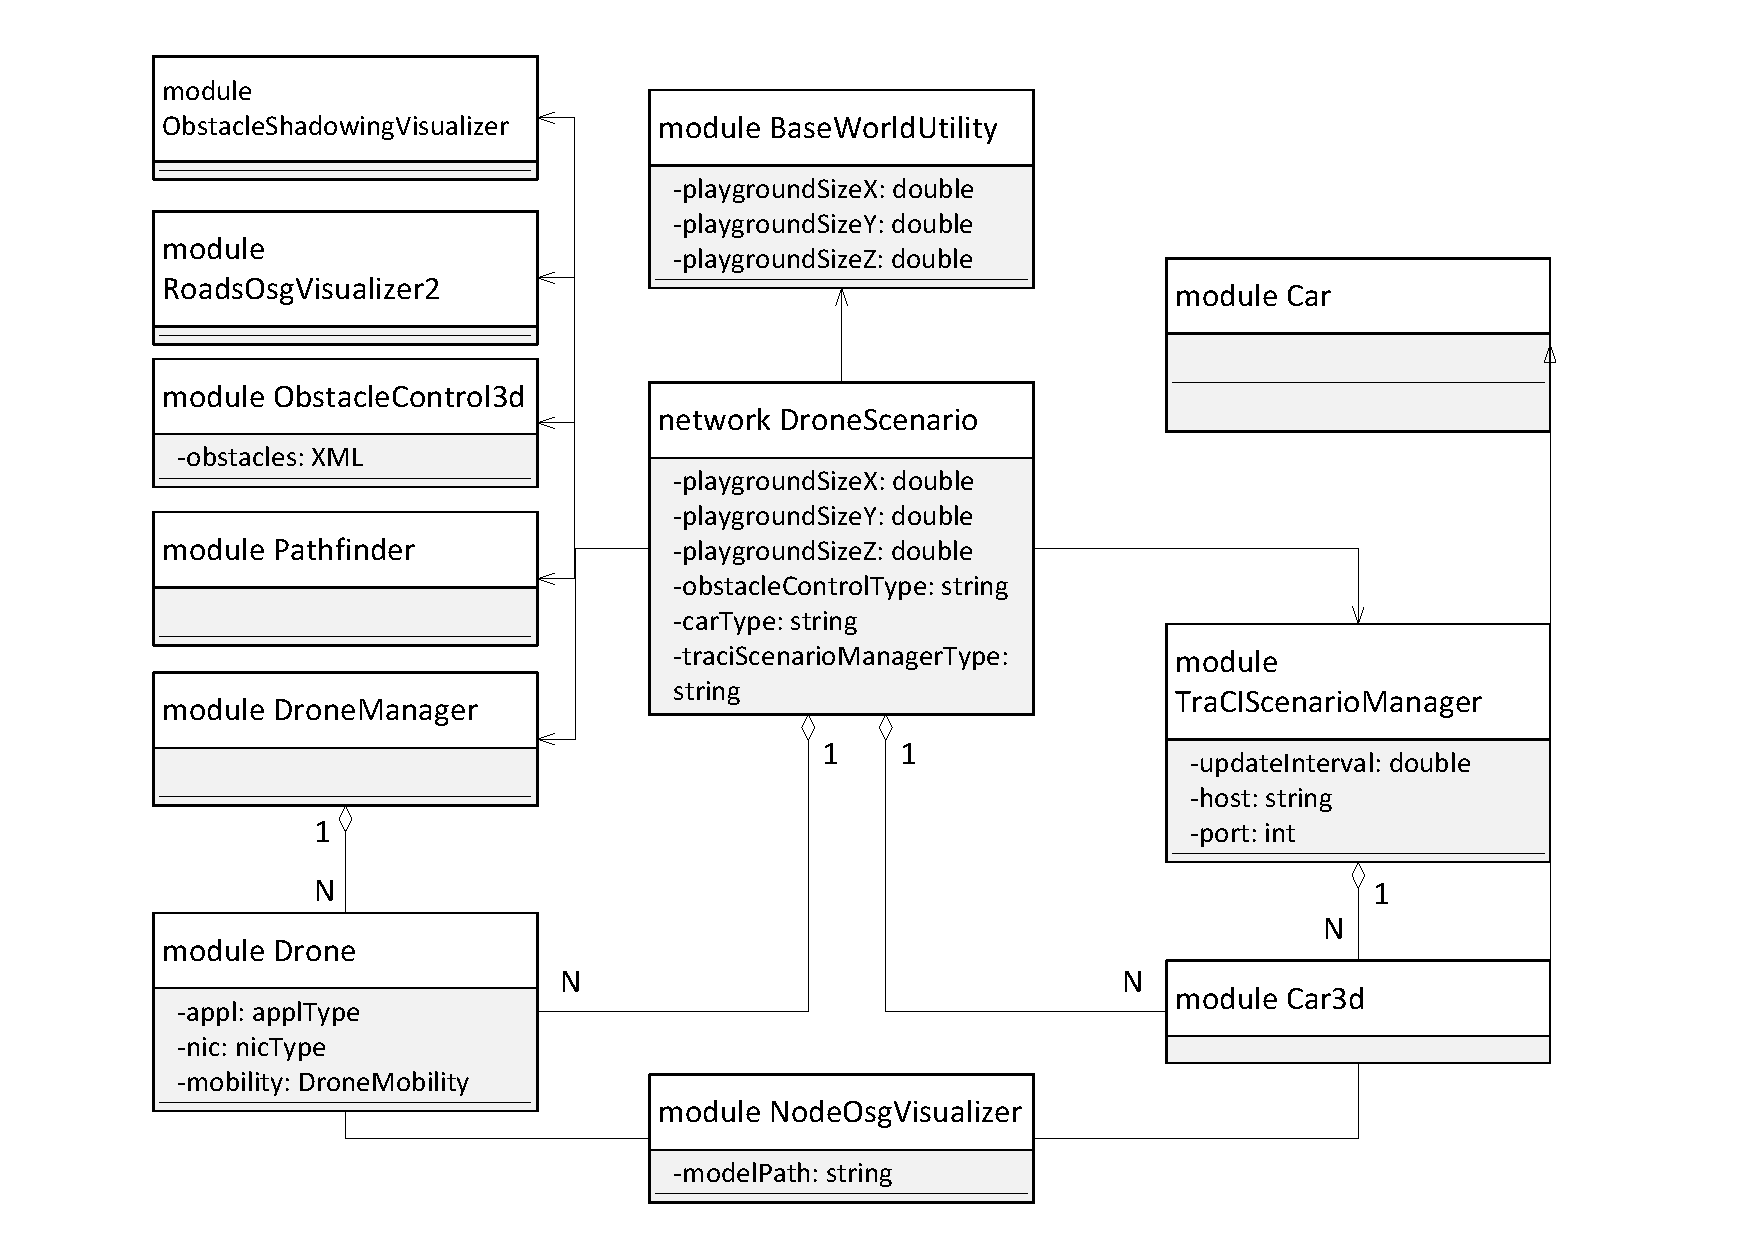
\includegraphics[width=1\textwidth]{figures/DroneScenario.pdf}
	\label{fig:dronescenarioned}
\end{figure}

\cref{fig:dronescenarioned} shows a simplified diagram of the network in my model, the scheme is analogues to \cref{fig:scenarioned} and is meant to show similarities and differences between my model in Veins' model.

In the following sections I will describe the differences in detail, explain how I have integrated in particular, drones, 3D-visualization and 3D-obstacle shadowing.

\section{Drones}

The first issue with implementing my scenario is that Veins does not support drones. Therefore, implementing drones was on of the first steps in my work. The easiest way to implement drones would be to reuse the existing Veins' code, that was used for vehicles. Therefore, drones will in fact only differ in their mobility, but in other things they will mostly share the code with Veins' vehicles.

\cref{fig:dronened} shows a simplified structure of the Drone.ned module. Like the Car.ned from Veins, Drone.ned uses a special submodule for moving in space. To improve simulation efficiency (i.e., to reduce the number of events), all drone movements are performed once every 1 second as part of the single event processing. The DroneManager.ned module is responsible for managing this event (scheduling and execution), as well as for creating and removing drones. Simply put, the DroneManager module creates a specified number of drones, and then sends a position update signal to each drone at a period of 1 second (configurable). 

DroneMobility module is based on Veins' LinearMobility with some minor changes. The biggest one: DroneMobility does not update itself. Instead, the DroneManager calls a special method that makes DroneMobility to update its position.

\begin{figure}
  	\caption{Simplified diagram of Drone module. Not all parameters connections are shown.}
	\centering
	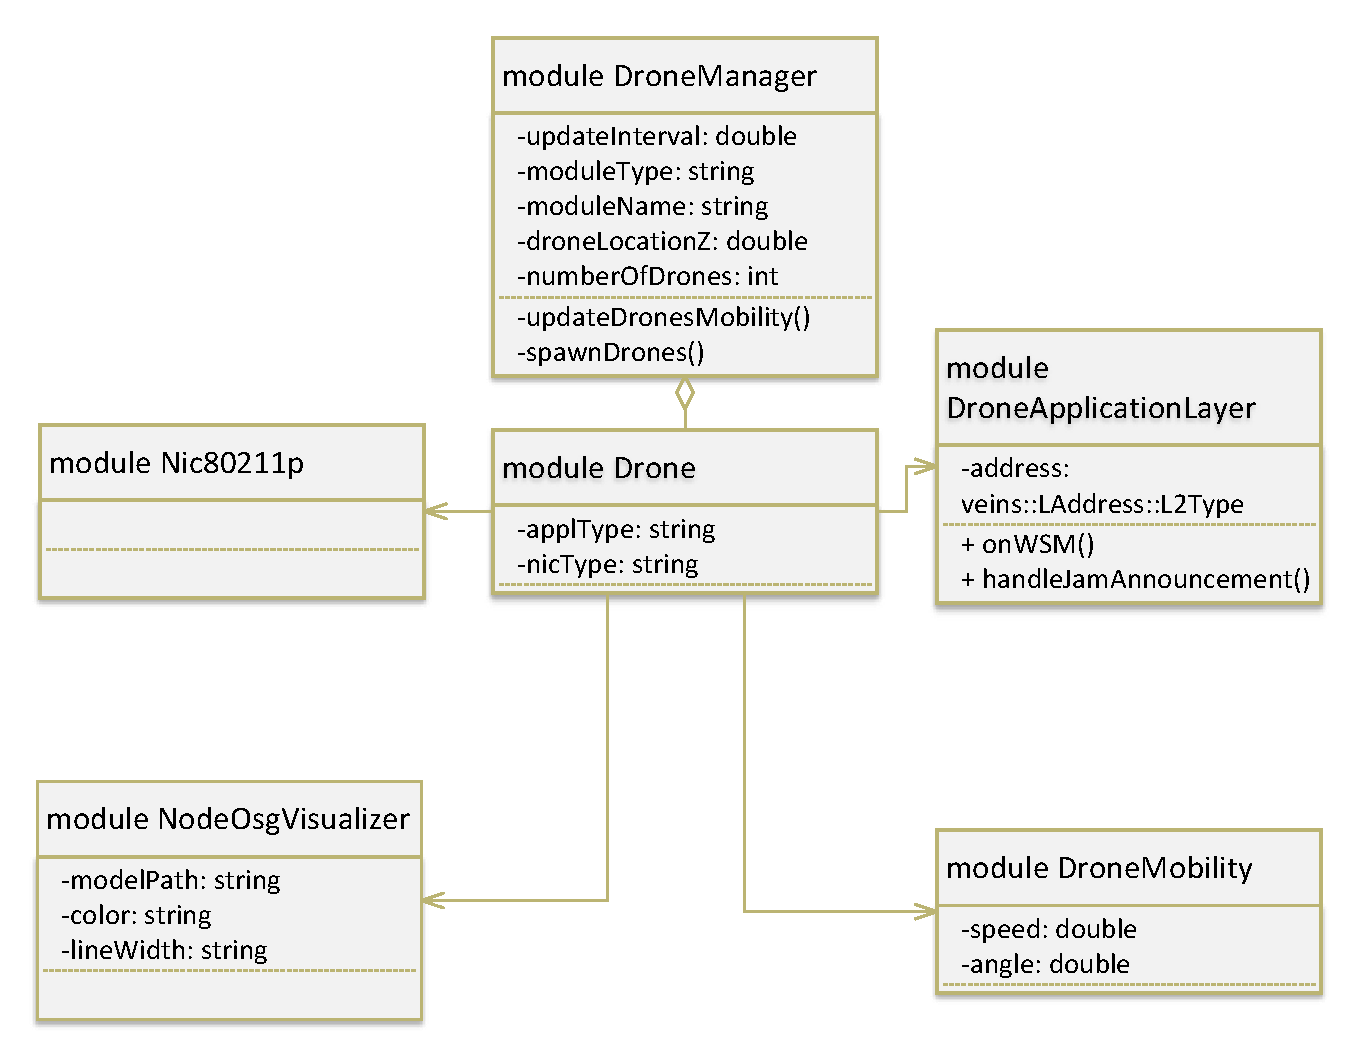
\includegraphics[width=1\textwidth]{figures/Drone.pdf}
	\label{fig:dronened}
\end{figure}


\section{BaseApplicationLayer}

To integrate the drones more easily, I decided to create an additional level of abstraction: BaseApplicationLayer (\cref{fig:baseapplicationlayer}), which will be common for drones and cars. This class is responsible for automatically assigning network addresses, for keeping track of statistics common to drones and cars, and, importantly, for decisions about relaying incoming messages. BaseApplicationLayer inherits from DemoBaseApplLayer, that is implemented in Veins.

\begin{figure}
  	\caption{Simplified diagram of BaseApplicationLayer. Not all parameters are shown. DemoBaseApplLayer is implemented in Veins \cite{demobaseappllayer}}
	\centering
	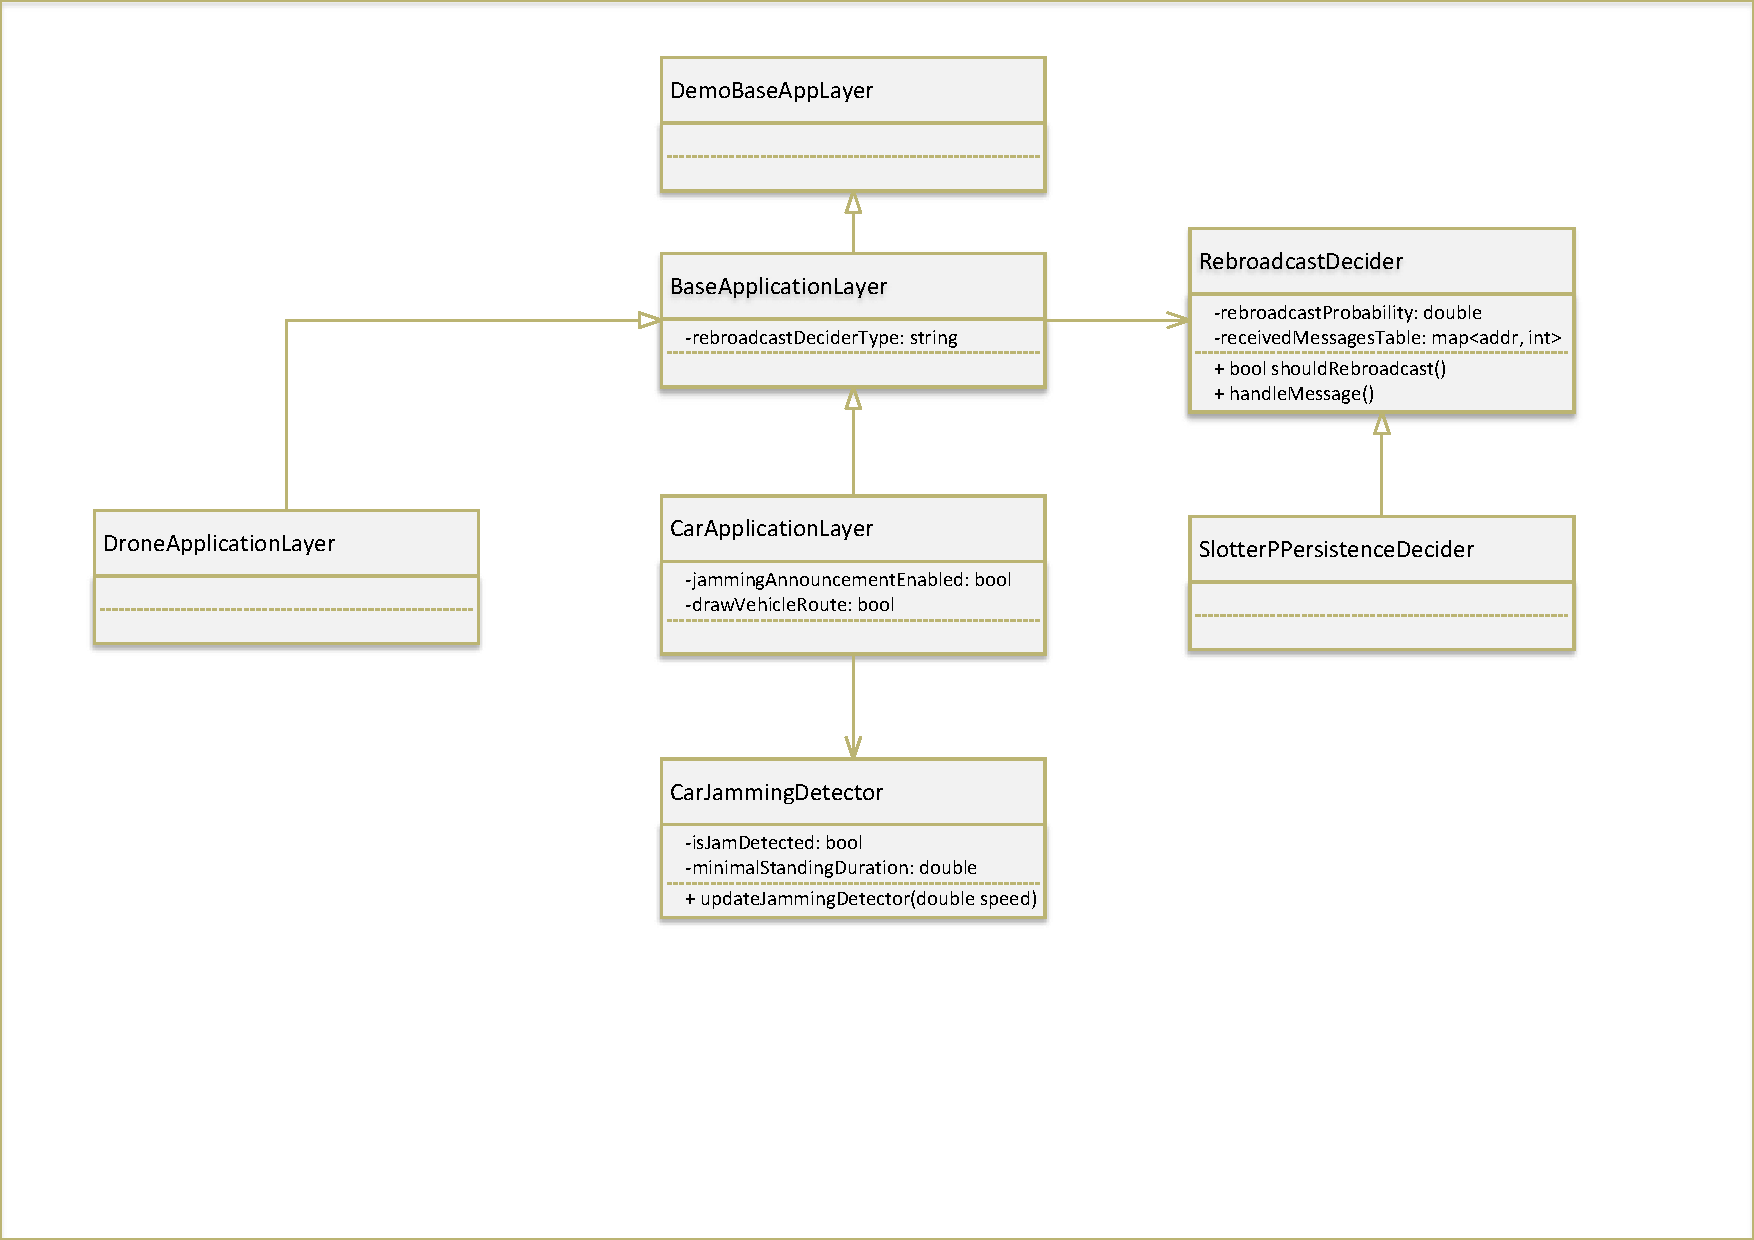
\includegraphics[width=1\textwidth]{figures/BaseApplicationLayer.pdf}
	\label{fig:baseapplicationlayer}
\end{figure}

The main reason for creating the BaseApplicationLayer is to unify the way how decision about rebroadcasting is made. BaseApplicationLayer holds a reference to a special object of class RebroadcastDecider, which in fact is a virtual class. This object decides whether to rebroadcast the message or not. How exactly it makes this decision for the vehicle or for the drone is irrelevant. The drone or vehicle only receives a decision from this object. So it is relatively easy to change the algorithm that decides whether to retransmit a message. Also it is easy to enable a specific algorithm for both drones and vehicles in the same manner.


\chapter{Evaluation}

\chapter{Conclusion}

\cleardoublepage

\listofabbreviations
\clearpage

\listoffigures
\clearpage

\listoftables
\clearpage

\printbibliography

\end{document}
